% $HeadURL$

\subsection{Glyph: \glyph{Tag}}
\label{sec:tag}

A \glyph{tag} is a named handle, or reference, to another \glyph{EPN} (\sect{EPNs}) or \glyph{compartment} (\sect{compartment}) \add{of the map}.
\add{Together with the \glyph{submap terminal} (\sect{submapTerminal}), it allows linking glyphs of a map to their counterpart in a submap.}
% \dogrusoz{I would replace "lying in a submap" with simply "in a submap".}
\corr{\glyph{Tags} are used to identify those elements in \glyph{submaps} (\sect{submap}).}{}

\begin{glyphDescription}

\glyphSboTerm Not applicable.

\add{
\glyphIncoming
One \glyph{equivalence arc} (\sect{equivalenceArc}).
}

\add{
\glyphOutgoing
None.
}

\glyphContainer A \glyph{tag} is represented by a \corr{rectangle}{rectangular shape} fused to an empty arrowhead, as \corr{illustrated}{shown} in \fig{tag}.
\corr{The flat edge opposite to the arrowhead should be aligned to the edge of the \glyph{submap} glyph, and from the middle of this edge should depart only one arc (see figure~\ref{fig:tag}).}{The incoming \glyph{equivalence arc} (\sect{equivalenceArc}) should be linked to the extremity of the arrowhead.}

\glyphLabel A \glyph{tag} is identified by a label \corr{placed in}{that is} \corr{an unbordered box containing}{} a string of characters \corr{.
The characters}{that} may be distributed on several lines to improve readability.
The \add{centre of the} label \corr{box} must be \corr{attached}{placed} \corr{to}{on} the centre of the \corr{container}{shape}.
The label may \corr{spill}{extend} outside of the \corr{container}{shape}.

\glyphAux 
\corr{A \glyph{tag} does not carry any auxiliary items}{None}.

\end{glyphDescription}

% \begin{figure}[htb]
% \centering
% 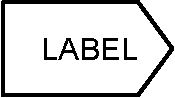
\includegraphics[scale = 0.3]{images/submapterminal}
% \caption{The \PD glyph for \glyph{tag}. This shows the
%   basic glyph and its correct usage within a \glyph{submap} glyph.     }
% \label{fig:tag}
% \end{figure}

% FIX 101717: images/tag
\begin{figure}[H]
  \centering
  \includegraphics{images/tag}
  \caption{The \PD glyph for \glyph{tag}.}
  \label{fig:tag}
\end{figure}

% The following is for [X]Emacs users.   Please leave in place.
% Local Variables:
% TeX-master: "../sbgn_PD-level1"
% End:

